\documentclass[11pt]{beamer}
\usetheme{AnnArbor}
\usepackage[utf8]{inputenc}
\usepackage[spanish]{babel}
\usepackage{amsmath}
\usepackage{xcolor}
\usecolortheme{spruce}
\usepackage{here}
\graphicspath{{../Images/}}
\usepackage{verbatim}
\usepackage{amsfonts}
\usepackage{marvosym}
\usepackage[marvosym]{tikzsymbols}
\usepackage{tikz}
\usepackage{tikzducks}
\usepackage{amssymb}
\usepackage{graphicx}
\usefonttheme{professionalfonts}
\author{HeNeos}
\title{Una introducción no formal a \LaTeX}
\institute[UNI]{Universidad Nacional de Ingeniería}
\begin{document}
\begin{frame}

\includegraphics[scale=0.05]{UNI}
\titlepage
\end{frame}
\begin{frame}{¿Qué es \LaTeX ?}
\LaTeX \, que se pronuncia como \textit{Lah-tech}, es un sistema de preparación de documentos para la composición tipográfica de alta calidad.\\[10pt]
{\LARGE ¡\LaTeX \, no es un procesador de textos!}\\[4pt]
En cambio, \LaTeX \, alienta a los autores a no preocuparse demasiado por la apariencia de sus documentos, sino a concentrarse en obtener el contenido correcto. \LaTeX \, se basa en la idea de que es mejor dejar el diseño del documento a los diseñadores de documentos y dejar que los autores sigan escribiendo documentos.\\[10pt]
{\LARGE \LaTeX \, es un sistema de preparación de documentos}\\[4pt]
\LaTeX \, es un sistema de composición tipográfica de alta calidad; incluye características diseñadas para la producción de documentación técnica y científica. \LaTeX \, es el estándar de facto para la comunicación y publicación de documentos científicos. \LaTeX \, está disponible como software libre.
\end{frame}
\begin{frame}
\frametitle{¿Por qué usar \LaTeX \, y no una alternativa WYSIWYG?}
WYSIWYG es el acrónimo de \textbf{W}hat \textbf{Y}ou \textbf{S}ee \textbf{I}s \textbf{W}hat \textbf{Y}ou \textbf{G}et ("\!\textit{lo que ves es lo que obtienes}"). Básicamente nos referimos a los procesadores de texto como Microsoft Word, OpenOffice, LibreOffice, etc.\\[20pt]
\LaTeX \, a diferencia de los anteriores mencionados no nos provee de un visualizador inmediato de lo que estamos escribiendo, pues este necesita compilar el fichero \texttt{.tex} mediante algunos \textit{métodos} para producir distintos archivos (\texttt{.dvi, .ps, .pdf})\\[6pt]
A primera vista, esto podría suponer una desventaja frente a los otros procesadores de texto habituales. Sin embargo, esta característica de \LaTeX \, permite a quien escribe un documento centrarse exclusivamente en el contenido.
\end{frame}
\begin{frame}
\frametitle{Ventajas de \LaTeX}
\begin{columns}[t]
\begin{column}{.48\linewidth}
\begin{block}{\LaTeX}
\begin{itemize}
\item Es \textit{open source} y es un software libre.
\item Es el estándar para la creación de documentos científicos y técnicos.
\item Facilidad al escribir expresiones matemáticas complejas.
\item El diseño del documento es semi-automático, permitiendo darle instrucciones muy básicas para su configuración.
\end{itemize}
\end{block}
\end{column}
\begin{column}{.48\linewidth}
\begin{block}{Microsoft Word}
\begin{itemize}
\item Requiere una licencia que debe ser renovada para utilizar el software.
\item Cada parte del documento tiene que ser personalizada por separado y manualmente.
\item No cuenta con un soporte para escribir texto matemático complejo.
\end{itemize}
\end{block}
\end{column}
\end{columns}
\end{frame}
\begin{frame}
\frametitle{Motivación para usar \LaTeX}
Con \LaTeX \, podemos lograr escribir expresiones matemáticas complejas de forma \textit{simple}, un ejemplo:
\begin{eqnarray}
\sum\limits_{n=1}^{\infty} \frac{\sigma_{a}(n) \sigma_{b}(n)}{n^s} =& \displaystyle{\frac{\zeta(s)\zeta(s-a)\zeta(s-b)\zeta(s-a-b)}{\zeta(2s-a-b)}} \\[4pt]
\notag \sigma_{x}(n) =& \sum\limits_{\mu=1}^{n} \mu^{x-1} \sum\limits_{\nu=1}^{\nu} \cos \frac{2\pi\nu n}{\mu}
\end{eqnarray}
O podríamos realizar diapositivas (como ésta \Winkey[1.2][yellow]), pósters o trípticos.
\end{frame}
\begin{frame}{Motivación para usar \LaTeX}
O también, podemos hacer gráficos vectoriales con TikZ que es un paquete de \LaTeX:
\begin{figure}[H]
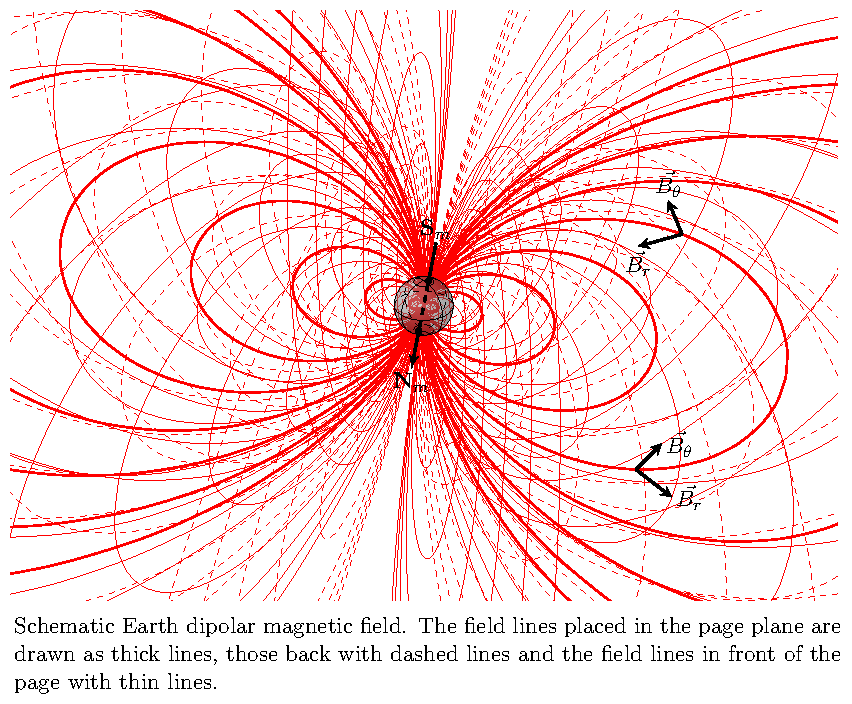
\includegraphics[scale=0.43]{dipolar-magnetic-field.pdf}
\caption{Campo magnético dipolar}
\end{figure}
\end{frame}
\begin{frame}
\frametitle{Motivación para usar \LaTeX}
Al ser open source, muchas personas han desarrollado varias \textit{implementaciones} no oficiales que podrían sernos útiles (o por lo menos, graciosas):
\begin{center}
\begin{tikzpicture}
\duck[body=yellow!50!red!20!white,
recedinghair=gray!50!white,
eyebrow,
tshirt=white!93!black,
jacket=red!50!black,
glasses=brown!70!lightgray,
book=\scalebox{0.5}{\TeX},
bookcolour=black!20!brown]
\end{tikzpicture}
\\Knuth Duck
\end{center}
\begin{center}
\begin{tikzpicture}
\colorlet{skin}{white!45!gray!80!green}
\duck[lightsaber, body=skin, bill=gray!80!green,
tshirt=brown!50!black, jacket=brown!30!gray]
\fill[skin,rounded corners=3] (0.44,1.70) -- (0.25,2)
-- (0.6,1.95);
\fill[skin,rounded corners=3] (1.34,1.60) --
(1.53,1.9) -- (1.16,1.85);
\end{tikzpicture}
\end{center}
\end{frame}
\begin{frame}[fragile]
\frametitle{Vale, me he convencido... pero, ¿cómo comienzo?}
Antes de empezar a escribir tu primer \begin{verbatim} \begin{document} \end{verbatim}
debes entender que aunque \LaTeX \, es una herramienta muy potente y puedes escribir toda clase de documentos con el, algunas veces resulta una mejor opción utilizar una herramienta Office.\\[28pt]
Bien, lo primero que necesitaremos serán las macros \TeX; para ello podemos instalar \href{https://miktex.org/download}{\textcolor{cyan}{\underline{MiKTeX}}} o \href{https://tug.org/texlive/}{\textcolor{cyan}{\underline{TeXLive}}}.\\[8pt]
Luego, necesitaremos un editor de texto dedicado a \LaTeX \,, personalmente les recomiendo \href{http://www.xm1math.net/texmaker/download.html}{\textcolor{cyan}{\underline{TeXMaker}}} pero pueden usar cualquiera de su agrado (tal vez alguien sabe codear en Vim... :0).\\[8pt]
Opcionalmente, pueden usar Overleaf, ShareLaTeX o Verbosus para escribir \LaTeX \, de forma online.
%\textcolor{cyan}{\underline{\url{http://www.latex-project.org/}}}
\end{frame}
\begin{frame}
\frametitle{Y ahora, ¿cómo aprendo a escribir en \LaTeX?}
Asiste a clases y practica mucho \Ninja[1.5][green!50][blue].\\ 
\begin{itemize}
\item Edición de textos científicos \LaTeX \, - \texttt{Borbón A., Alexander}
\item La introducción no tan corta a \LaTeX \, - \texttt{Oetiker, Tobías}
\item \texttt{CTAN}
\item \texttt{Blogs, blogs y más blogs}
\end{itemize}
\vfill
Nos vemos en la próxima clase.\\[70pt]
Beamer hecho con \texttt{AnnArbor}.
\end{frame}
\end{document}
